73. \begin{figure}[ht!]
\center{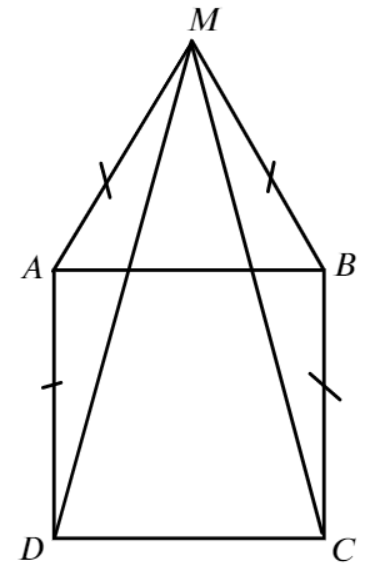
\includegraphics[scale=0.35]{g73.png}}
\end{figure}\\
Так как $ABCD$ квадрат, а треугольник $AMB$ равносторонний, имеем $AD=BC=AB=AM=BM,$ поэтому треугольники $DAM$ и $CBM$ являются равнобедренными. Углы $DAM$ и $CBM$ равны $90^\circ+60^\circ=150^\circ,$ а значит $\angle ADM=\angle BCM=(180^\circ-150^\circ):2=15^\circ.$ Таким образом, $\angle MDC=\angle MCD-90^\circ-15^\circ=75^\circ,\ \angle DMC=180^\circ-75^\circ-75^\circ=30^\circ.$\\
